% doc type
\documentclass[12pt]{article}

% set up supplemental section
\newcommand{\beginsupplement}{%
	\setcounter{table}{0}
	\renewcommand{\thetable}{S\arabic{table}}%
	\setcounter{figure}{0}
	\renewcommand{\thefigure}{S\arabic{figure}}%
}

% format page, paragraph
\usepackage[margin=1in]{geometry}
\usepackage{lineno}
\linenumbers
\usepackage{setspace}
\doublespacing
\usepackage[utf8]{inputenc}
\usepackage[hidelinks]{hyperref}
\usepackage{authblk}

% bib - uses better biblatex
\usepackage[style=apa,backend=biber]{biblatex}
\addbibresource{./Zotero_adr_dwi.bib}

% figures and tables
\usepackage{graphicx}
\graphicspath{ {./} }
\usepackage{multirow}
\usepackage[table,xcdraw]{xcolor}
\usepackage{url}
\usepackage{float}
\usepackage{longtable}

% code
\usepackage{listings,lstautogobble}
\lstset{language=R,
	basicstyle=\small\ttfamily,
	otherkeywords={0,1,2,3,4,5,6,7,8,9},
	morekeywords={TRUE,FALSE},
	deletekeywords={data,frame,length,as,character},
	autogobble=true
}
\renewcommand\lstlistingname{R Code}

% math
\usepackage{amsmath}
\usepackage{caption}
\DeclareCaptionType{equ}[R Code][]

% title page info
\title{Longitudinal study of concussion-related diffusion MRI changes in college athletes}
\date{}

\author[1,*]{Nathan M. Muncy}
\author[1]{Heather C. Bouchard}
\author[1]{Aron K. Barbey}

\affil[1]{Center for Brain, Behavior and Biology, University of Nebraska-Lincoln, Lincoln, Nebraska, USA}
\affil[*]{Corresponding author.	Email: nmuncy2@unl.edu}

% start document
\begin{document}

% title page
\maketitle
\pagebreak


% abstract page
\begin{abstract}

% TODO: Update, finalize.

Sports-related traumatic brain injuries affect 1.6-3.8 million individuals in the US each year, and diffusion weighted imaging can measure the complex timeline of resulting axolemmal changes. Such longitudinal data is difficult to model statistically, however, given the high-dimensionality, semi-parametric and interdependent scalar values, and non-linear spatial (within-tract) and temporal (across visit) properties. Proposal: hierarchical generalized additive models (HGAMs) are well-suited to fit such data with the requisite flexibility and sensitivity to investigate (a) the spatial and temporal changes of white matter tracts, and (b) how such changes relate to diagnostic assessments. Methods: we utilized MRI and IMPACT data collected from 67 college athletes (9 female, age=19.43[1.68]) at three visits: start-of-season, post-concussion, and return-to-play. Diffusion tensors were modeled via constrained spherical deconvolution and probabilistic tractography from pyAFQ yielded 100 scalar values per white matter bundle. Results: By fitting the scalar profiles with longitudinal HGAMs we detected within-tract changes as a function of visit, revealing distinct patterns of post-injury disruption and recovery. Critically, it is unlikely that such changes would have been detected with standard techniques given their linear assumptions and limited dimensionality. Further, we examined whether these evolving diffusion metrics correlated with cognitive outcomes using HGAM tensor product interaction smooths and found moderate evidence linking white matter alterations to IMPACT composite scores. Merit: HGAMs offer a powerful framework to capture the complex progression of brain injury. Our findings suggest that HGAMs enhance our understanding of the spatiotemporal dynamics of brain injury and may enable more accurate tracking of injury and recovery.

\end{abstract}

\vfill
KEYWORDS: DWI, MRI, GAM, TBI\\
\pagebreak


\section{Introduction}
\label{sec:intro}
Introduction here.

% TODO: (Heather?) Epidemilogic description of TBI in US, athletes
% TODO: mTBI sequelae description
% TODO: DWI and mTBI
% TODO: Modeling DWI, issues
% TODO: Purpose - (a) extend GAMs for longitudinal DWI, (b) tensor product interaction smooths for multi-modal analyses


\section{Methods}
\label{sec:meth}

\subsection{Participants}
\label{ssec:meth-part}
Participants were recruited from men's football and women's soccer programs at the University of Nebraska-Lincoln, resulting in the enrollment of 69 (9 female, age = 19.36 $\pm$1.67, range = 17-24) National Collegiate Athletic Association (NCAA) athletes. Additional demographic metrics (e.g. race, ethnicity, SES) are omitted to protect participant confidentiality as University athletes are public figures and identification may cause deleterious consequences. Due to the limited number of females, and the sport-sex confound, we combined all participants into a single group. Institutional Review Board approval was obtained at the outset of the study, and prior to beginning experimental procedures participants completed informed consent and assent. Magnetic Resonant Imaging (MRI) and clinical assessment (ImPACT) data were acquired during three sessions: enrollment at the beginning of the season (baseline, Base), within 48 hours of diagnosed concussion (post-concussion, Post), and prior to return-to-play (RTP). As MRI and ImPACT (below) data were gathered separately, a number of participants did not contribute MRI and/or ImPACT data across one or more of the sessions. This resulted in the following final session counts: Base = 67 MRI (9 female), 61 ImPACT (5 female), Post = 65 MRI (8 female), 48 ImPACT (3 female), and RTP = 56 MRI (7 female), 32 ImPACT (2 female).


\subsection{ImPACT}
\label{ssec:meth-imp}
Description of ImPACT.

% TODO: (Heather) Description of ImPACT collection and items.


\subsection{MRI Protocol}
\label{ssec:meth-mri}
Magnetic Resonance Imaging data were collected on a 3-Tesla Siemens MAGNETOM Skyra scanner at the Center for Brain, Behavior and Biology (University of Nebraska-Lincoln) utilizing a 32-channel coil. For each of three sessions (Base, Post, and RTP), participants contributed T1 and diffusion weighted images (T1w, DWI). T1w Multi-Echo Magnetization Prepared - RApid GRadient Echo (MEMP-RAGE) structural scans were acquired with the following parameters: TR = 2530 ms, TE = 1.69, 3.55, 5.41, and 7.27 ms, flip angle = 7$^{\circ}$, voxel size = 1 mm$^3$, FoV = 256 $\times$ 256, slices = 176 interleaved. DWI scans were acquired via TR = 3000 ms, TE = 95 ms, flip angle = 90$^{\circ}$, voxel size = 1.719 $\times$ 1.719 $\times$ 2.4 mm$^3$, 134 slices, multi-band acceleration factor = 3, directions = 128, bandwidth = 1500 Hz/Px, shells = 1 (b-value = 1000 s/mm$^2$), reference volumes = 6 (b-values = 0 s/mm$^2$; b$_0$). A set of field maps for the DWI scans were collected using the same acquisition direction (anterior-posterior; AP) and reversed (posterior-anterior; PA).

% TODO verify coil type


\subsection{MRI Data Processing}
\label{ssec:meth-mri-proc}
Preprocessing and modeling of the DWI data were conducted using FSL v6.0 \parencite{jenkinson2012Fsl} and PyAFQ v1.3.6 \parencite{kruper2021EvaluatingReliabilityHuman,yeatman2012TractProfilesWhite}. First, b$_0$ volumes and acquisition parameters were extracted and combined from the AP and PA field maps, and \lstinline{topup} used the resulting AP-PA b$_0$ file to calculate a distortion correction matrix. Next, a brain mask was constructed via \lstinline{bet}, and then preprocessing of the DWI data was conducted with \lstinline{eddy_openmp}, which incorporated the distortion correction matrix, brain mask, and a volume-acquisition parameter mapping index to produce motion- and distortion-corrected diffusion images.

Whole-brain tractography was computed from the preprocessed DWI by PyAFQ. Constrained spherical deconvolution was used to derive the fiber orientation distribution function (fODF) of each voxel, where constrained-positivity regularization = 1, minimum amplitude $\tau$ = 0.1, mean gray matter diffusivity = 0.0008, mean CSF diffusivity = 0.003, 600 fODF iterations, and spherical harmonics order = 8. Resulting fODFs of each voxel were then utilized to probabilistically generate fiber maps, using one seed per voxel for each dimension, a maximum turning angle of 30$^\circ$, step size = 0.5 mm, and a length range = 50-250 mm. The resulting fibers were parcellated into individual tracts via \textit{a priori} inclusion (waypoint) and exclusion regions of interest \parencite{wakana2007ReproducibilityQuantitativeTractography}. These tracts were then compared to a fiber probability map \parencite{hua2008TractProbabilityMaps} and any fibers which traverse low-probability spaces were removed from the tract. Further, any fibers with a length 3+ standard deviations from the tract average, or 4+ standard deviations from the average path centroid, were removed as well. Lastly, each tract was then resampled into 100 equidistant nodes (according to a Mahalanobis distance metric) from which averaged diffusion values and scalars were calculated. Specifically, for each tract node we extracted averaged axial diffusivity ($\lambda_\parallel$; AD), radial diffusivity ($(\lambda_{\perp1}+\lambda_{\perp2})/2$; RD), mean diffusivity ($(\lambda_\parallel+\lambda_{\perp1}+\lambda_{\perp2})/3$; MD), and fractional anisotropy (FA). It was determined upon review of the 28 parcellated tract bundles that bilateral posterior arcuate and vertical occipital tracts were not well identified across all subjects and sessions, accordingly analyses only included the remaining 24 white matter tracts. Finally, as scalar values approach zero at the start and end of tracts due to fiber fanning, fitting the distribution becomes rather problematic. We removed the first and last 10 nodes and were subsequently able to fit the data well, and we note that this clipping of the ends is in addition to that already performed by the PyAFQ software.

% TODO: Cite that CSD, prob tract are better for TBI?


\subsection{GAM specification}
\label{ssec:meth-gam}

% TODO: are these two paragraphs better in the intro? Maybe a brief description goes in intro.

Generalized additive models (GAM) are an extension of general linear models capable of modeling high-dimensional data which contain non-linear relationships. Where regression models fit data with a linear (or higher-order polynomial) function, GAMs construct a smooth curve to fit data from a set of basis functions (i.e. splines). Such a smooth can capture complex X-Y relationships that would be underfit by models with linear assumptions. Further, high dimensional relationships can be modeled via 3-dimensional smooths (i.e. membrane), termed a `tensor product interaction smooth', or with hypersurfaces for higher dimensions \parencite{baayen2020IntroductionGeneralizedAdditive}. Such capabilities have made GAMs useful in fields such as ecology ([CITE]), paleontology \parencite{simpson2018ModellingPalaeoecologicalTime}, and linguistics ([CITE]), which often model complex data in high dimensions or across multiple factors, and researchers using MRI techniques are beginning to adopt the method ([CITE]). We recently demonstrated their applicability to modeling DWI scalar data \parencite{muncy2022GeneralAdditiveModels}, and here we extend GAMs to model high-dimensional, longitudinal, multimodal data.

Hierarchical GAMs (HGAMs; \cite{pedersen2019HierarchicalGeneralizedAdditive}) allow for model fits at both global and group levels. That is, it is possible to model both the X-Y relationship that is shared across all levels of a factor (global smooth) and differences that factor levels (group smooths) may have from the global smooth. Further, it is not required that each level of smooth (global, group) contain the same `wiggliness' in the X-Y relationships. Separate smooth curves and wiggliness terms at different factor levels of HGAMs is highly relevant in modeling concussion-related changes within white matter tracts, as the global smooth of the tractometric profile (i.e. scalar values across all nodes) can effectively be held constant when modeling potential changes across session, and independent wiggliness terms may capture scalar changes unique to one time point. Further, tensor product interaction terms can be utilized to build multimodal models, investigating the relationship of the tractometric profile with independent metrics such as the ImPACT composite scores. Accordingly, such a model would be capable not only of detecting changes within a tract that result from concussion, but also how such changes relate to clinical assessments. Finally, and critically, HGAMs facilitate conducting longitudinal, whole-brain analyses on tractometric profiles as data from all tracts and across all time points can be included in the same model. Such a specification allows for within-subject pooling of variance across both tract and time. Where modeling individual tracts results in a creeping Type-I error and the corresponding corrections, injury (and subsequent recovery) may affect multiple tracts within a subject and such shared variance would be lost when investigating tracts individually. By including all tracts and time points, HGAMs have the capability to not only reduce Type-I but also Type-II errors. All GAMs were specified using the \lstinline{mgcv} package version 1.9-1 \parencite{wood2017GeneralizedAdditiveModels} in R version 4.3.3 \parencite{rcoreteam2023LanguageEnvironmentStatistical}.

% TODO: include DWI scalar distribution (and plot) to visualize tractometric profile? Cite a yeatman tractometry paper?


\subsubsection{Longitudinal difference model}
\label{sssec:meth-gam-ldi}
To investigate within-tract injury- and recovery-related FA changes we specified an HGAM to test for Post and RTP tract FA differences from Base. First, we calculated the Post-Base and RTP-Base changes in FA ($\Delta$FA). While including original FA values would be ideal, propagating ordered factors (Base $<$ Post $<$ RTP) across an interaction with another factor (tract) loses the original ordered structure; ordered factors would be necessary to investigate differences from baseline instead of merely the interaction with session. Next, we calculated the session comparison $\times$ tract interaction term as \lstinline{mgcv::bam} does not currently support modeling smooths by factor interactions. $\Delta$FA values were modeled as a function of tract node using thin-plate regression splines (R Code \ref{code:gam-ldi}) and a basis dimensionality of 15 was determined sufficient to fit the tract curves (\lstinline{gam.check(fit_LDI)}). Subjects were treated as a random effect, thereby allowing each subject to have their own intercept across all levels of the factors, the $\Delta$FA distribution was well-fit by a Gaussian distribution with an identity link function, fast Residual Error of Maximum Likelihood (fREML) was used as the smoothing parameter estimation method, and 12 threads were used in the computation (run time $\approx$ 45 minutes). Input data consisted of the 24 tracts with good segmentation across all subjects. Notably, we did not include a global smooth for this model, as the $\Delta$FA profile would differ for each tract, and we specified that each tract would have its own wiggliness term; essentially this is a longitudinal model of FA differences which references model `I' in \textcite{pedersen2019HierarchicalGeneralizedAdditive}.

\begin{equ}[H]
	\begin{lstlisting}
		fit_LDI <- mgcv::bam(
		  delta_fa ~ s(subj_id, by=tract_scan, bs="re") +
		    s(node_id, by=tract_scan, bs="tp", k=15) +
		    tract_name+sess_comp+tract_scan,
		  data=df,
		  family=gaussian(),
		  method="fREML",
		  nthreads=12
		)
	\end{lstlisting}
	\caption{$\Delta$FA values are modeled as a function of tract node with thin-plate regression smooths for each tract, accounting for the within-subject factors of tract and session and using separate wiggliness terms for each tract. \lstinline{delta_fa} = RTP-Base and Post-Base FA differences, \lstinline{subj_id} = subject identifier factor, \lstinline{node_id} = node identifier integer, \lstinline{tract_name} = tract identifier factor, \lstinline{sess_comp} = session comparison factor (RTP-Base, Post-Base), and \lstinline{tract_scan} = interaction of \lstinline{tract_name} and \lstinline{sess_comp}.}
	\label{code:gam-ldi}
\end{equ}


\subsubsection{Longitudinal tract model}
\label{sssec:meth-gam-lgio}
The model specified in R Code \ref{code:gam-ldi} effectively models the entire longitudinal dataset of $\Delta$FA values, allowing for pooling for variance within a subject across tract and session, not requiring a multiple comparison correction for modeling all tracts. But as the $\Delta$FA calculation required data at time points A and B, the analysis was restricted by missing data. As essentially a post-hoc analysis to further interrogate tract differences across session, and also what change in scalar (e.g. increased RD) drove the difference in FA, individual tracts were modeled with a longitudinal HGAM with terms for global and group smooths (R Code \ref{code:gam-lgio}). Tract FA values were fit by a beta distribution with a logit link function, AD and RD values were fit with a Gaussian distribution and identity link function, and a gamma distribution with a logit link function fit the MD values. Subjects were again treated as a random effect, with separate intercepts for each scan (Base, Post, RTP), group smooths were allowed their own wiggliness parameter, and the colinearity of global and group smooths was controlled by the `m' parameter. Such a model is similar to model `GI' in \textcite{pedersen2019HierarchicalGeneralizedAdditive}. Finally, an ordered session factor was included to test for difference in Post and RTP scalar values from Base. Such a model is particularly useful as the test statistic, which describes the flatness of the smooth, provides information about changes from Base values rather than deflections from zero. A model which fits group smooths for each session is provided in Supplemental Materials (Supplemental R code \ref{supp-code:gam-lgi}).

\begin{equ}[H]
	\begin{lstlisting}
		df$scanOF <- factor(df$scan_name, ordered=T)
		fit_LGIO <- mgcv::bam(
		  <scalar> ~ s(subj_id, scan_name, bs="re") +
		    s(node_id, bs="tp", k=15, m=2) +
		    s(node_id, by=scanOF, bs="tp", k=15, m=1),
		  data=df,
		  family=<family>,
		  method="fREML",
		  nthreads=4
		)
	\end{lstlisting}
	\caption{Tract scalars are modeled as a function of tract node with thin-plate regression splines using both global and group (\lstinline{scan_name}) smooths as well as individual group wiggliness. An ordered factor of scan session was used to compare Post and RTP to Base. \lstinline{<scalar>} = relevant DWI metric (AD, RD, MD, or FA), \lstinline{scan_name} = session identifier factor (Base, Post, RTP), \lstinline{scanOf} = ordered factor of \lstinline{scan_name}, \lstinline{<family>} = relevant family and link function for scalar distribution.}
	\label{code:gam-lgio}
\end{equ}


\subsubsection{Longitudinal tract interaction model}
\label{sssec:meth-gam-lgio-intx}
As noted above, GAMs are capable of modeling higher-dimensional, non-linear interactions through tensor product interaction smooths and hypersurfaces, a property which make them particularly relevant for multimodal research. We used such a model to test whether concussion- and recovery-related changes in tract scalars related to changes in ImPACT composite and total symptom scores (R code \ref{code:gam-lgio-intx}), thereby potentially linking damage within a specific region of a tract to changes in assessment metrics. Tract scalars were modeled as a function of both tract node and ImPACT measure, and the node-ImPACT interaction term was specified such that each session (Base, Post, RTP) would have a different scalar-node-ImpACT interaction surface. We note the decrease in basis dimensionality for the ImPACT measures thin-plate regression splines from the default value, and that fitting the tensor product interaction smooth also benefited from a slightly higher basis dimensions term for the tract node term. Finally, as above (Section \ref{sssec:meth-gam-lgio}), an ordered factor for session was included in order to test whether the Post and RTP interaction surfaces differed from that of Base; a model with separate interaction surfaces is provided in Supplemental Materials (Supplemental R code \ref{supp-code:gam-lgi-intx}).

\begin{equ}[H]
	\begin{lstlisting}
		df$scanOF <- factor(df$scan_name, ordered=T)
		fit_LGIO_intx <- mgcv::bam(
		  <scalar> ~ s(subj_id, scan_name, bs="re") +
		    s(node_id, bs="tp", k=15, m=2) +
		    s(imp_meas, by=scan_name, bs="tp", k=5) +
		    ti(node_id, imp_meas, bs=c"tp","tp"), k=c(20,5), m=1) +
		    ti(
		      node_id, imp_meas, by=scanOF,
		      bs=c("tp","tp"), k=c(20,5), m=1
		    ),
		  data=df,
		  family=<family>,
		  method="fREML",
		  nthreads=4
		)
	\end{lstlisting}
	\caption{Tract scalars are modeled as a function of separate 2D node and ImPACT smooths as well as a 3D tensor product interaction surface, with ordered factors used to compare Post and RTP surfaces to Base. \lstinline{imp_meas} = ImPACT composite or total symptom measure.}
	\label{code:gam-lgio-intx}
\end{equ}


\subsubsection{ImPACT model}
\label{sssec:meth-gam-impact}
The relationship between session (Base, Post, RTP) and ImPACT composite metrics (verbal memory, visual memory, visual motor, impulse control, and reaction time) and total symptom scores were modeled with GAMs to test for changes across assessment session. As with tract scalar profiles, GAMs were employed as (a) non-linear trends are expected in such metrics, and (b) they can model the semi-parametric distributions encountered in several of the metrics. Each ImPACT metric was fit as a function of assessment number, using integer values rather than categorical Base, Post, and RTP (Supplemental R Code \ref{supp-code:gam-impact}); such a specification allowed for modeling evolving changes in assessment metrics rather than comparing main effects across factor levels. Verbal and visual memory composites were converted to proportion scores and modeled with a beta distribution and logit link function, visual motor and reaction time were best fit with Gaussian distributions and identity link functions (despite the skewness), and a negative binomial distribution with log link function fit the impulse control and total symptoms well.

When specifying models, whether with ImPACT or DWI data, model fits were reviewed and assessed via \lstinline{mgcv:gam.check()}, and the selection of competing models was aided by \lstinline{itsadug::compareML()}. Pipeline and statistical code, information about their respective environments, and curated data are available at the project repository: \url{https://github.com/nmuncy/adr_dwi}.


\section{Results}
\label{sec:res}

\subsection{ImPACT}
\label{ssec:res-imp}
ImPACT assessment smooths (Section \ref{sssec:meth-gam-impact}) were extracted and plotted for visualization purposes (Figure \ref{fig:imp-gam}). All models except for impulse control detected a significant interaction between ImPACT metric and assessment number. Visual memory, reaction time, and total symptoms had patterns consistent with concussion-related deficits at Post and subsequent recovery at RTP (visual memory: $F_{(1.94, 1.99)}$ = 8.59, \textit{p} $<$ .001; reaction time: $F_{(1.91, 1.99)}$ = 6.18, \textit{p} $<$ .01; total symptoms: $F_{(1.98, 1.99)}$ = 28.74, \textit{p} $<$ .0001). We also note that total symptoms at RTP were much lower than at Base (Figure \ref{fig:imp-gam}, bottom right). Conversely, while verbal memory and visual motor tests indicate significant non-flatness (verbal memory: $F_{(1.82, 1.96)}$ = 4.34, \textit{p} = .028; visual motor: $F_{(1.86, 1.97)}$ = 8.19, \textit{p} $<$ .001), their values did not differ between Base and Post while RTP scores were significantly better. This pattern possibly reflects a lack of sensitivity at Base and/or practice effects. Finally, impulse control was unchanged (i.e. flat) as a function of assessment ($F_{(1.0, 1)}$ = .003, \textit{p} = .95).

\begin{figure}[H]
	\centering
	\fbox{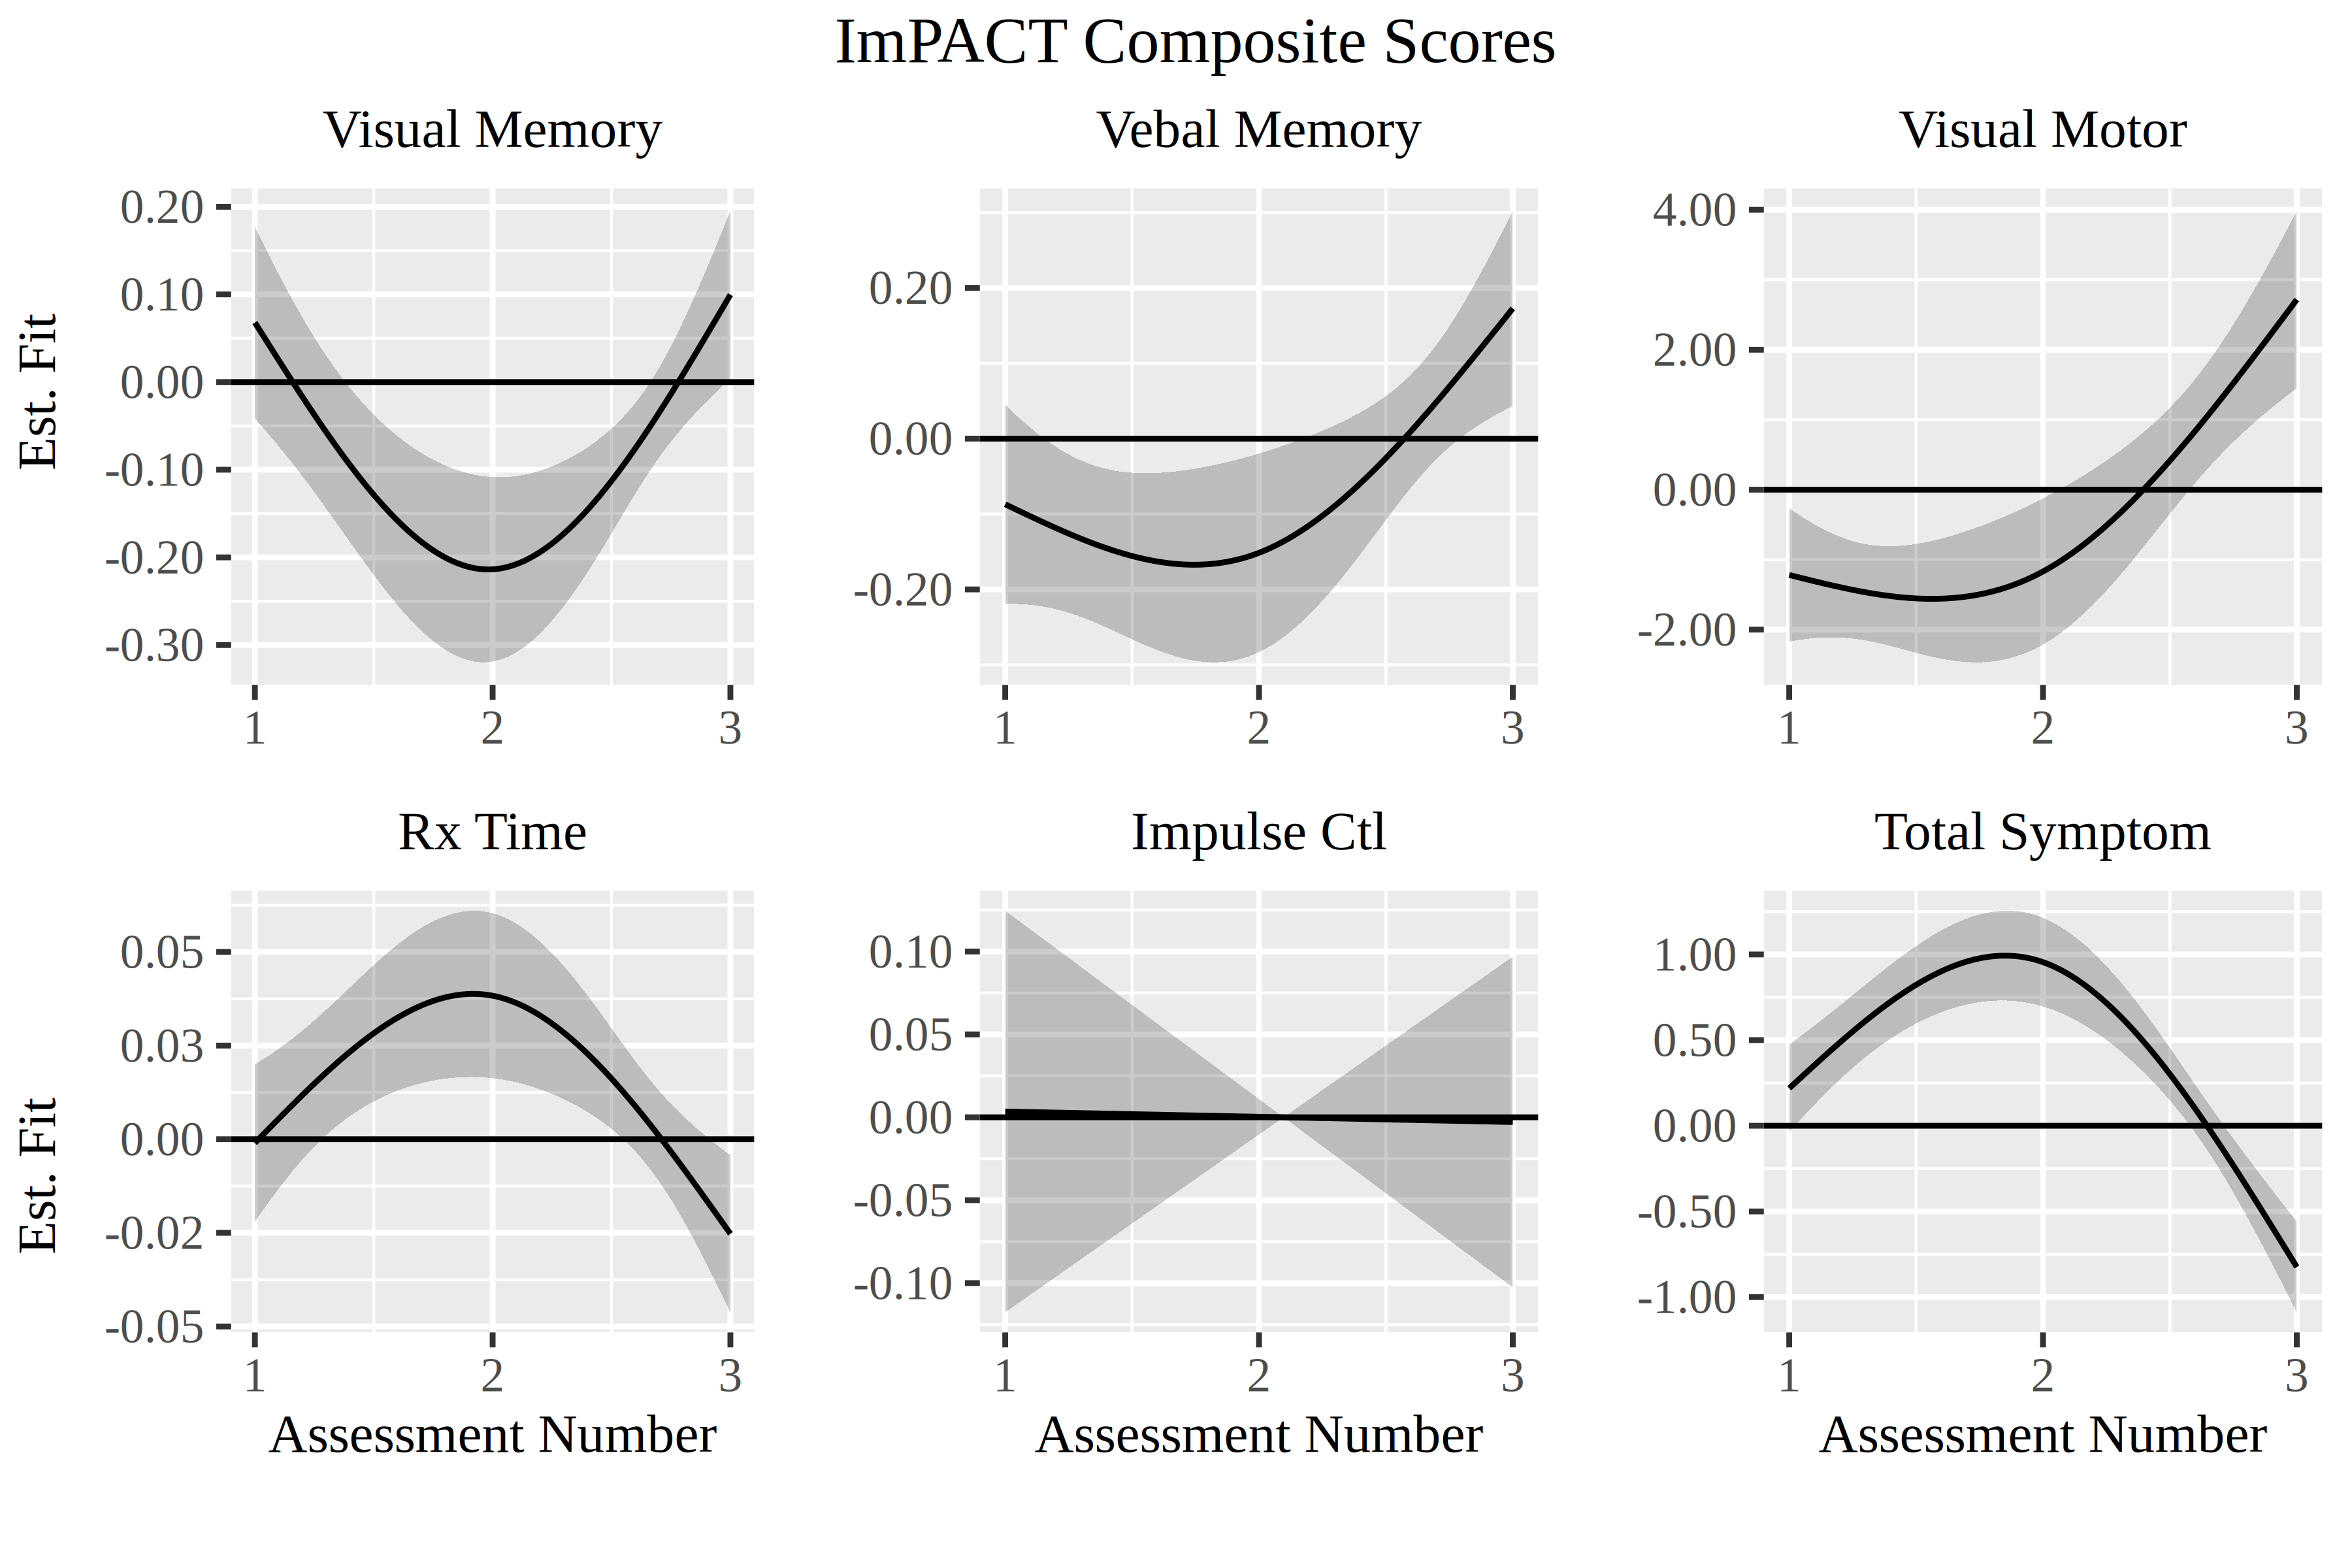
\includegraphics{fig_impact_gam.png}}
	\caption{GAM smooths for ImPACT composite and total symptom scores. Assessment numbers where the confidence interval does not include 0 indicate significant changes. Visual memory, reaction time, and total symptoms showed worsening and then recovery (U-shapes) while verbal memory and visual motor scores were better at assessment 3. Impulse control did not change across assessments. Assessment number 1=Base, 2=Post, 3=RTP. Rx Time = reaction time, Impulse Ctl = impulse control.}
	\label{fig:imp-gam}
\end{figure}


\subsection{DWI Tracts}
\label{ssec:res-dwi-tract}

\subsubsection{Whole-Brain Analyses}
\label{sssec:res-dwi-tract-wba}
The longitudinal, whole-brain difference model (Section \ref{sssec:meth-gam-ldi}) produced tract difference smooths for Post-Base and RTP-Base $\Delta$FA values (Figure \ref{fig:ldi-gam}, top and middle). Surprisingly, test statistics for all smooths indicate significant non-flatness, suggesting that at least some regions of each tract differed significantly between Base and Post as well as Base and RTP. We note that in interpreting GAM coefficients, the magnitude of the effect is equally relevant to the test statistic of non-flatness (F-stat). For instance, the corpus callosum orbital (CCorb, left, green) had a much larger magnitude compared to another, equally `significant' tract (corpus callosum temporal (CCtemp), pink). Nevertheless, it is well established that mTBI is associated with negative diagnostic readings \parencite[e.g.][]{klein2019PrevalencePotentiallyClinically}, and we expected to only find changes to scalar values in regions commonly associate with traumatic axonal injury (e.g. splenium of corpus callosum, left of midline (CCsp, CCpp)).

\begin{figure}[H]
	\centering
	\fbox{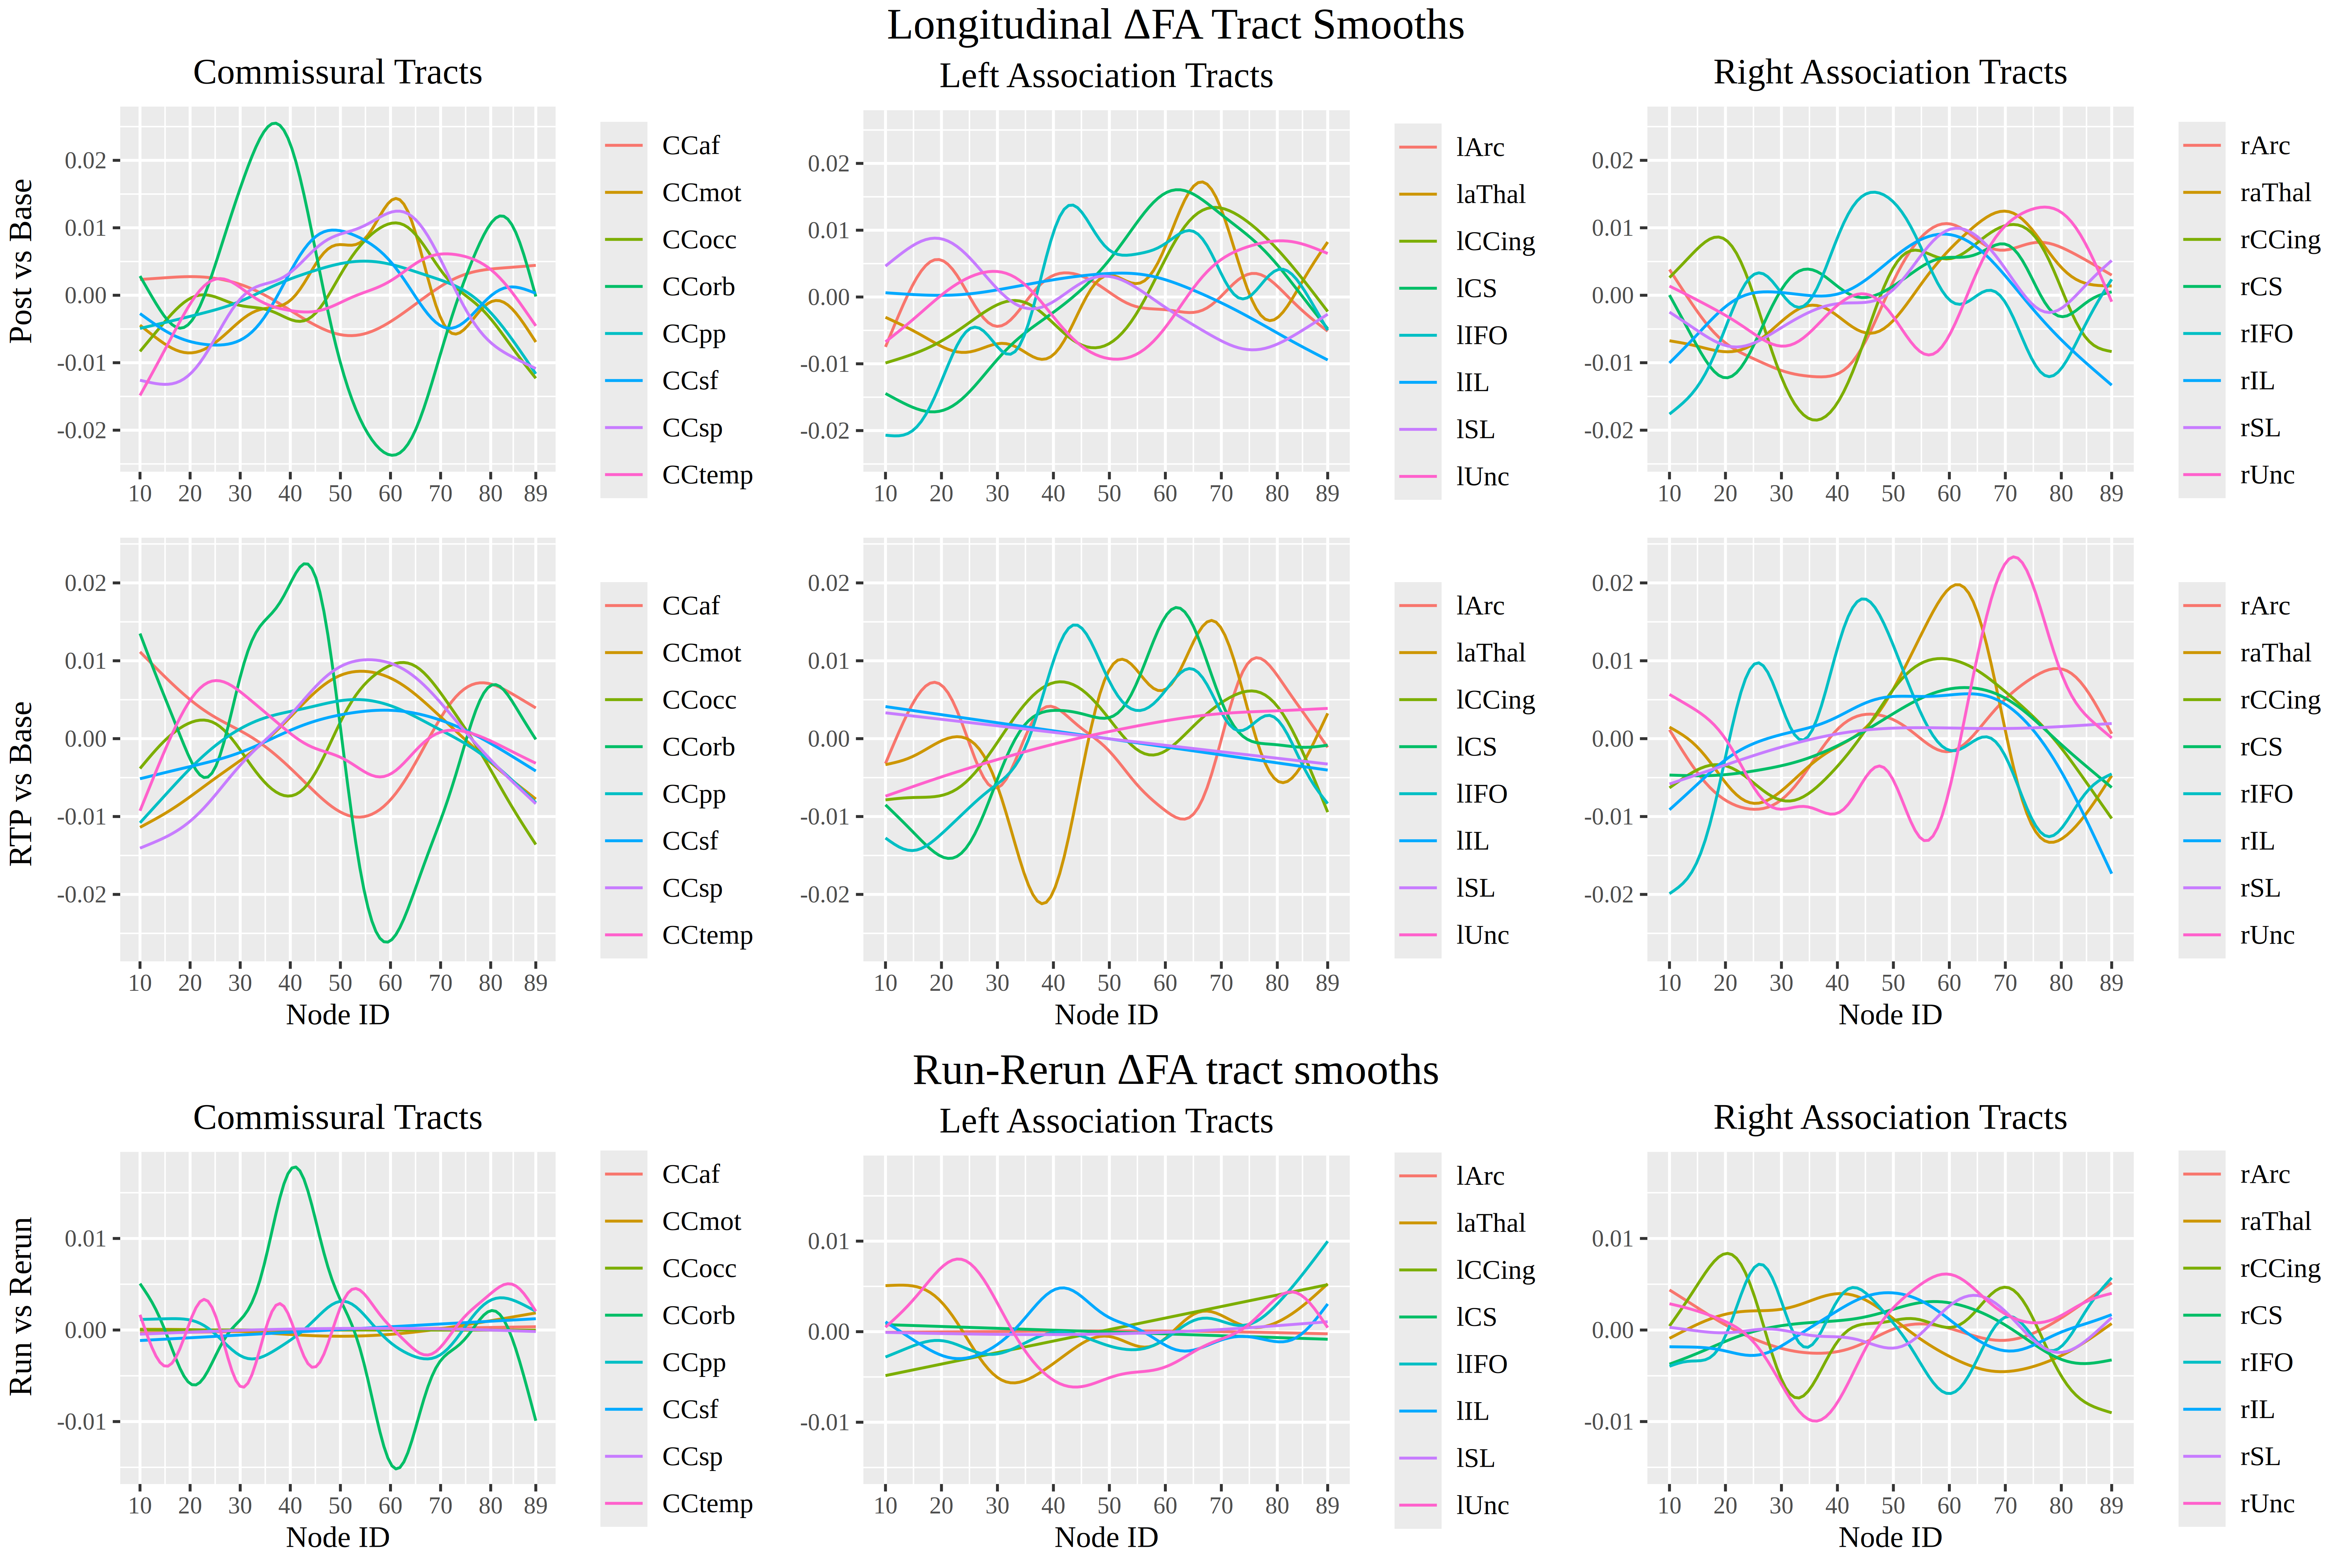
\includegraphics[scale=0.5]{fig_LDI_DI_rerun.png}}
	\caption{HGAM smooths of tract FA differences by node for comparisons against Base (top, middle) and run-rerun (bottom). Top: $\Delta$FA-Node smooths of Post-Base, deflections from zero here may be indicative of concussion-related changes. Middle: $\Delta$FA-Node smooths of RTP-Base, smaller deflections here than Post-Base may be indicative of recovery-related changes (and the converse for greater deflections). Bottom: $\Delta$FA-Node smooths of Run-Rerun, indicative of algorithmic variance by tract. Left: Corpus callosum tracts, middle: left hemisphere tracts, right: right hemisphere tracts. CCaf = anterior forceps, CCmot = motor, CCocc = occipital, CCorb = orbitalis, CCpp = posterior parietal, CCsf = superior frontal, CCsp = superior parietal, CCtemp = temporal. Arc = arcuate, aThal = anterior thalamic, CCing = cingulum (cingulate portion), CS = corticospinal, IFO = inferior fronto-occipital, IL = inferior lateral, SL = superior lateral, Unc = uncinate. Node IDs are counted posterior-anterior or right-left. Confidence intervals were omitted for visual clarity.}
	\label{fig:ldi-gam}
\end{figure}

As tractometry was conducted on each session via PyAFQ, one potential source of variance is algorithmic (i.e. pipeline) run-rerun (test-retest) stability, particularly given our use of probabilistic tractography. Previous work has demonstrated high test-retest reliability metrics for PyAFQ \parencite{kruper2021EvaluatingReliabilityHuman}, which also noted tract-dependent reliability metrics that averaged around 86\%. We note that concussion-related scalar changes may not be as large as 14\%, particularly at the group level due to injury heterogeneity. To quantify the amount of algorithmic variance in our data, we reran tractography on the Base session and calculated Run-Rerun $\Delta$FA values for each subject's tract profiles. The Run-Rerun $\Delta$FA were modeled with a non-longitudinal variant of R Code \ref{code:gam-ldi} (Supplemental R Code \ref{supp-code:gam-di}). Resulting smooths (Figure \ref{fig:ldi-gam}, bottom) illustrate the amount of algorithmic variance that can be expected for each tract, where some tracts have demonstrably high variance (e.g. CCorb) while others are more stable (CCsf). Corresponding test statistics identified a number of tracts which did not significantly differ between run and rerun (CCaf, CCmot, CCocc, CCsp, lArc, lCS, and lSL) and for the remaining tracts we considered any difference to be related to concussion or recovery if the magnitude of the effect was larger than that of run-rerun.

% TODO: analyses just focus one stable tracts?
% TODO: Supplemental table of LDI, DI stats.

\subsubsection{Tract-Specific Analyses}
\label{sssec:res-dwi-tract-tsa}

% TODO: Table of tract statistics
% TODO: for table, detail \lstinline{s(node_id):scanOFpost} and \lstinline{s(node_id):scanOFrtp}

As a selection of tracts did not show significant algorithmic variance, we selected to focus on a subset commonly implicated in sports-related concussion, specifically the splenium (superior parietal corpus callosum; CCsp), forceps minor (anterior frontal corpus callosum, CCaf), left corticospinal tracts (lCS), and left arcuate (lArc). Individual models were used to fit the FA, MD, AD, and RD scalars for each tract to test for Post and RTP differences from Base (R Code \ref{code:gam-lgio}). Test statistics for Post  and RTP difference smooths [REF TABLE] indicate that all smooths differed significantly from Base in at least one region of nodes, save for lCS AD smooth (both Post and RTP were identical to Base) as well as the lArc Post FA smooth (Figure \ref{fig:lgio-gam}).

\begin{figure}[H]
	\centering
	\fbox{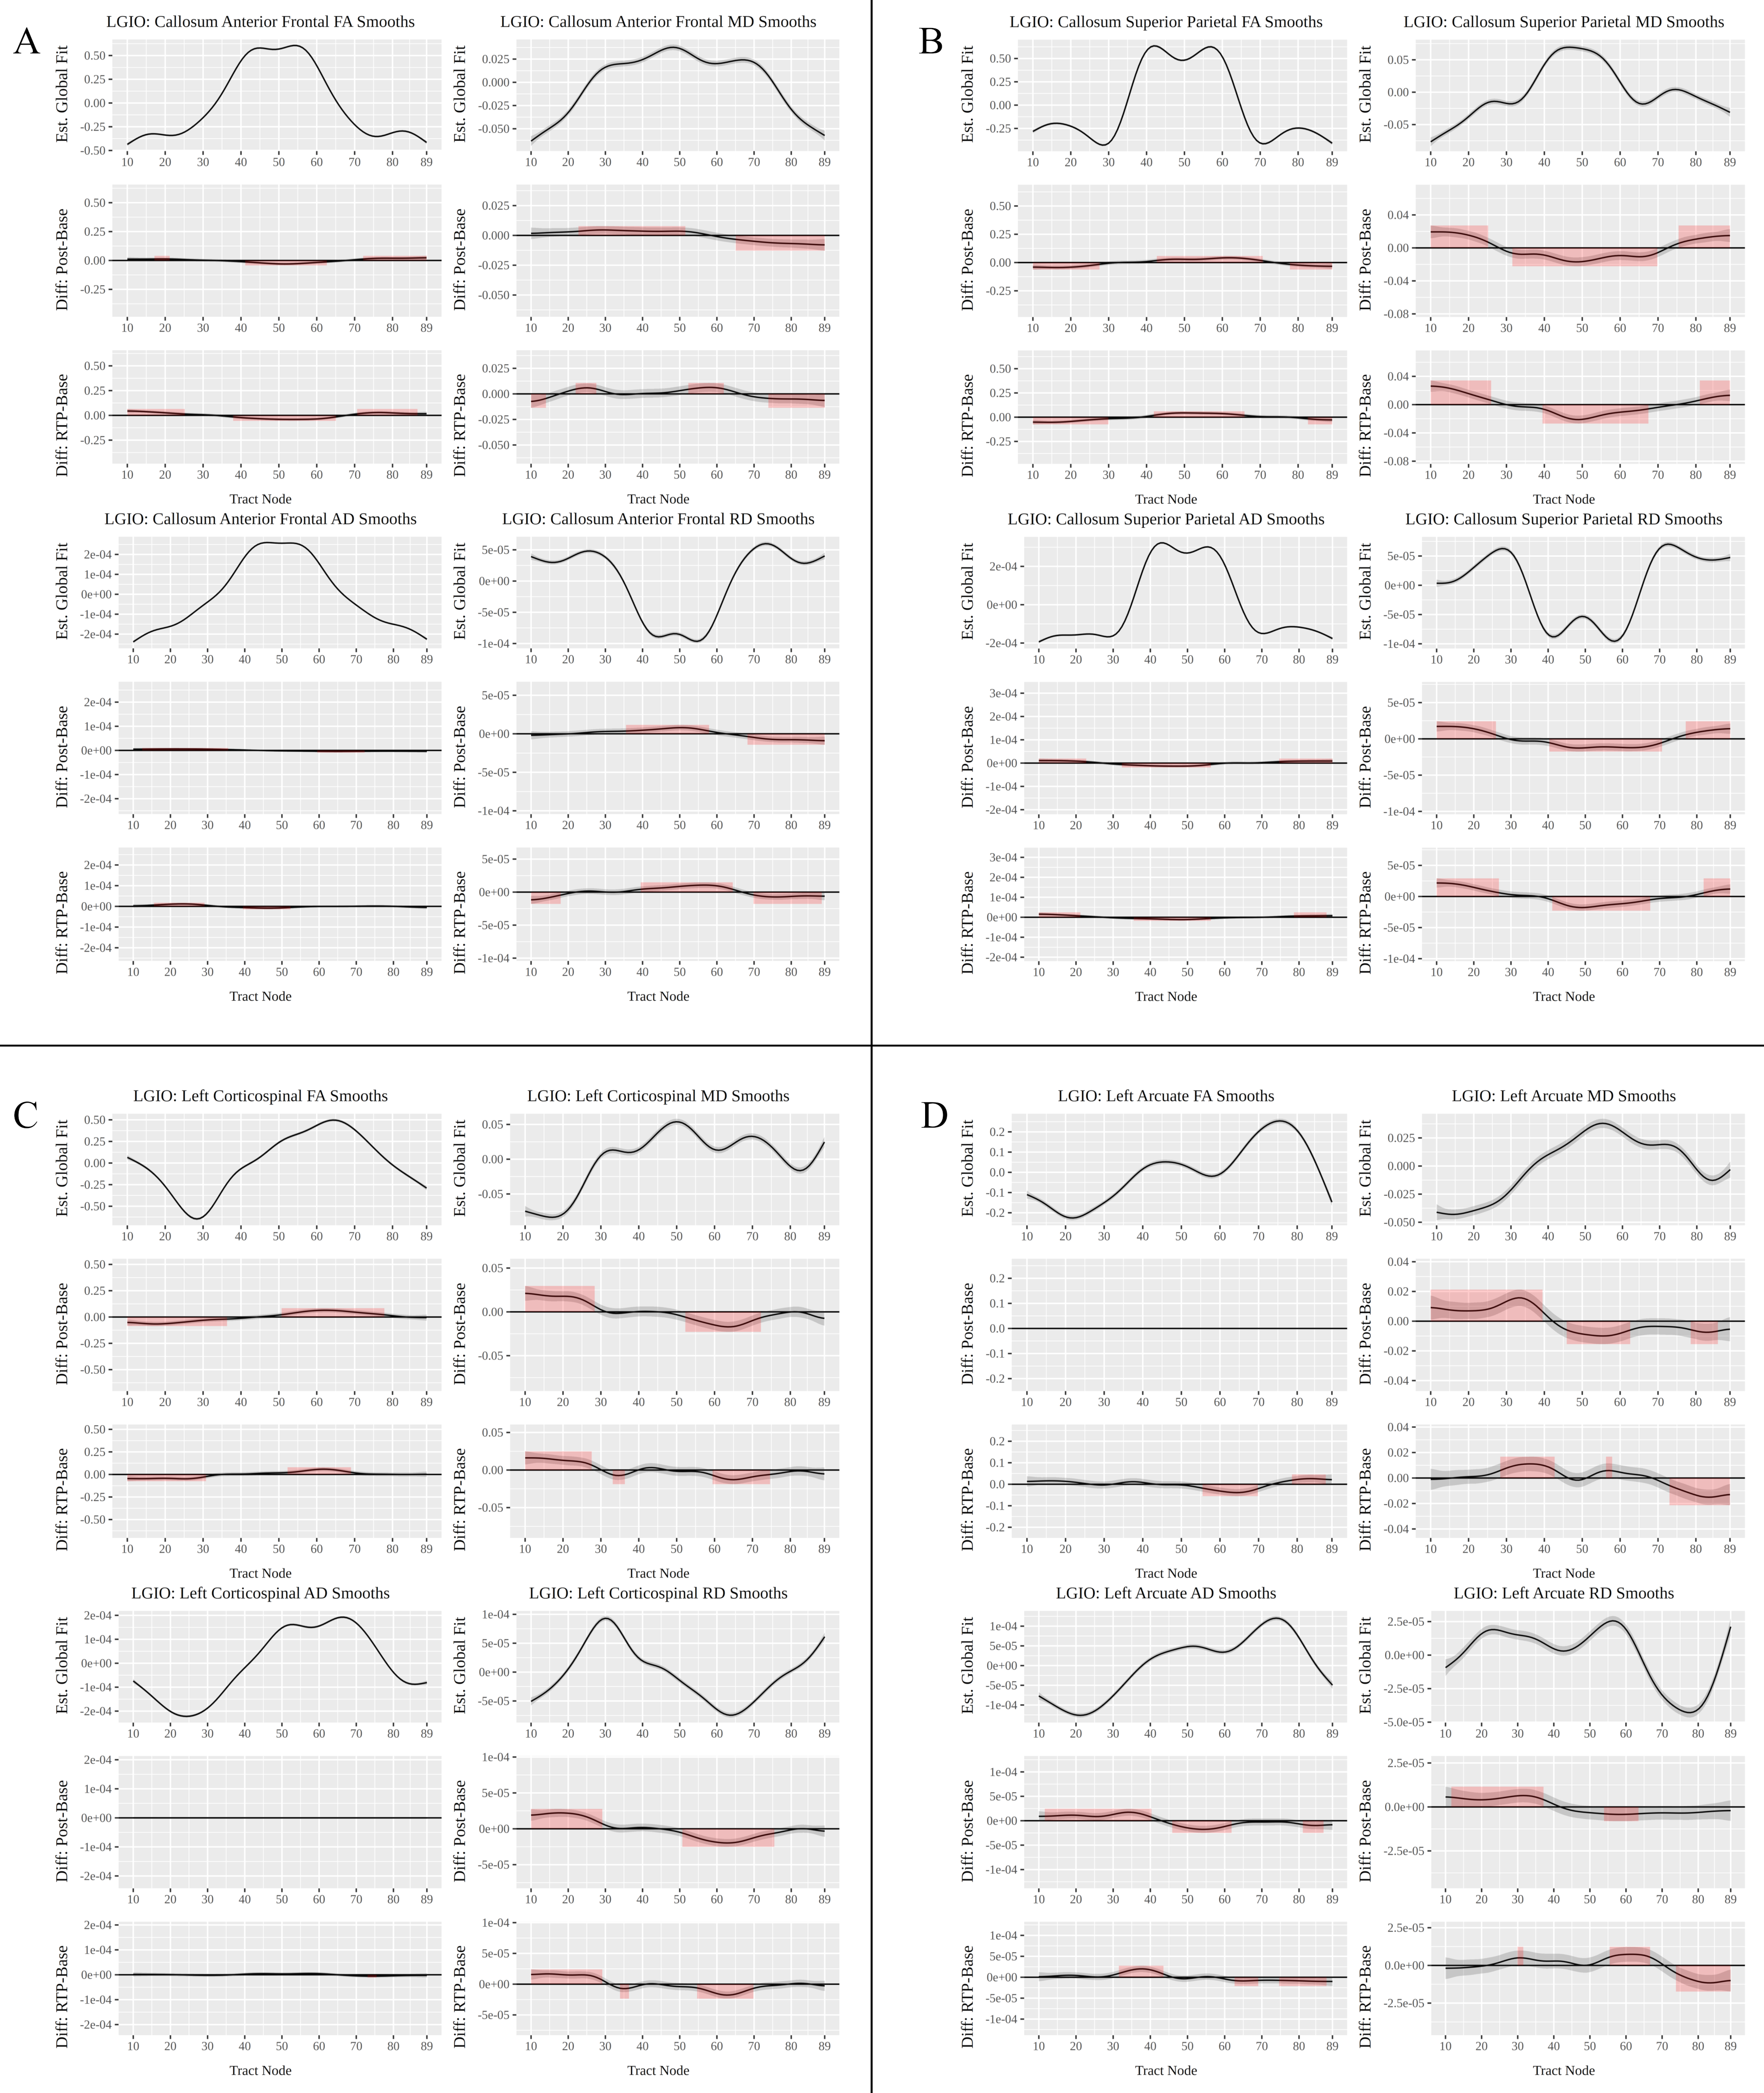
\includegraphics[scale=0.10]{fig_lgio_smooths.png}}
	\caption{Longitudinal HGAM smooths modeling DWI scalar as a function of node. Each model fit both the global tractometric profile (global smooths) and how sessions differed from the global (group smooths). Specifically, session was treated as an ordered factor so resulting session smooths are a `difference from Base' smooth. For example, left arcuate Post FA values did not differ from Base (D, top right) while RTP had lower FA values than base around node 65. Each quadrant contains global and session smooths for FA (top left), MD (top right), AD (bottom left), and RD (bottom right). A: Corpus Callosum Anterior Frontal (forceps minor), B: Corpus Callosum Superior Parietal, C: left Corticospinal, D: left Uncinate tract. Red boxes indicate nodes where smooths differ statistically from the reference group (Base).}
	\label{fig:lgio-gam}
\end{figure}

At Post, both callosal tracts (CCaf, CCsp) showed changes to FA values left of midline (approximate nodes 50-60), changes which were driven in large part by RD. Increased RD in CCaf, without changes in RD, resulted in a lower FA value relative to Base at Post. Conversely, decreased RD values were associated with increased FA values in CCsp.


% TODO: detail rx bx FA and o/scalars


\subsection{DWI Tracts Interactions - ImPACT}
\label{ssec:res-dwi-imp}
Description of DWI - ImPACT interaction.

% TODO: Motivate select tracts
% TODO: LGI_intx, LGIO_intx GAMs tracts - vis_mem?


\subsection{DWI Tracts Interactions - Time}
\label{ssec:res-dwi-time}
Description of DWI-time interaction.

% TODO: DI_time GAM results - rSLF?


\section{Discussion}
\label{sec:disc}
Discussion.

% TODO: Summary/recap
% TODO: Interpret main findings
% TODO: Advocate HGAMs for mTBI research, reference AFQ-Insight?
% Limitations: Interpretation of statistic (flatness and LGI, LGIO models), all data in one model - underfit certain profiles, scan-rescan variance in addition to algorithmic, heterogeneity of injury and insufficient sample size to cluster symptom profiles.


% acknowledgment page
\section*{Acknowledgments}
\label{sec:ack}
People. Grant.

% TODO: ariana for consulting


% write bibliography
\pagebreak
\printbibliography
\pagebreak


% make supplemental
\section{Supplemental Materials}
\label{sec:supp-materials}
\beginsupplement
Supplemental Materials.


\begin{equ}[H]
	\begin{lstlisting}
		fit_LGI <- mgcv::bam(
		  <scalar> ~ s(subj_id, scan_name, bs="re") +
		    s(node_id, bs="tp", k=15, m=2) +
		    s(node_id, by=scan_name, bs="tp", k=15, m=1),
		  data=df,
		  family=<family>,
		  method="fREML",
		  nthreads=4
		)
	\end{lstlisting}
	\caption{Tract scalars are modeled as a function of tract node with thin-plate regression splines using both global and group (\lstinline{scan_name}) smooths as well as individual group wiggliness. \lstinline{<scalar>} = relevant DWI metric (AD, RD, MD, or FA), \lstinline{scan_name} = session identifier factor (Base, Post, RTP), \lstinline{<family>} = relevant family and link function for scalar distribution.}
	\label{supp-code:gam-lgi}
\end{equ}


\begin{equ}[H]
	\begin{lstlisting}
		fit_LGI_intx <- mgcv::bam(
		  <scalar> ~ s(subj_id, scan_name, bs="re") +
		    s(node_id, bs="tp", k=15, m=2) +
		    s(imp_meas, by=scan_name, bs="tp", k=5) +
		    ti(
		      node_id, imp_meas, by=scan_name,
		      bs=c("tp","tp"), k=c(20,5), m=1
		    ),
		  data=df,
		  family=<family>,
		  method="fREML",
		  nthreads=4
		)
	\end{lstlisting}
	\caption{Tract scalars are modeled as a function of separate 2D node and ImPACT smooths as well as a 3D tensor product interaction surface. \lstinline{imp_meas} = ImPACT composite or total symptom measure.}
	\label{supp-code:gam-lgi-intx}
\end{equ}


\begin{equ}[H]
	\begin{lstlisting}
		fit_G <- mgcv::bam(
		  imp_meas ~ s(subj_id, bs="re") +
		    s(num_assess, bs="tp", k=3),
		  data=df,
		  family=<family>,
		  method="fREML"
		)
	\end{lstlisting}
	\caption{ImPACT metrics modeled as a function of number of assessments using a single global smooth. \lstinline{imp_meas} = ImPACT composite or total symptom score, \lstinline{num_assess} = assessment number (1=Base, 2=Post, 3=RTP).}
	\label{supp-code:gam-impact}
\end{equ}


\begin{equ}[H]
	\begin{lstlisting}
		fit_DI <- mgcv::bam(
		  delta_fa ~ s(subj_id, by=tract_name, bs="re") +
		    s(node_id, by=tract_name, bs="tp", k=15) +
		    tract_name,
		  data=df,
		  family=gaussian(),
		  method="fREML",
		  nthreads=12
		)
	\end{lstlisting}
	\caption{Run-Rerun $\Delta$FA values were modeled with node smooths for each tract.}
	\label{supp-code:gam-di}
\end{equ}

\subsection{Tables}
\label{ssec:supp-tables}
Supplemental Tables.


\subsection{Figures}
\label{ssec:supp-figures}
Supplemental Figures.


\end{document}